\section{Обзор существующих проблем и решений}
\label{Solution} \index{Chapter 4}

\subsection{Lost in the middle}
\label{subsec:lost_in_the_middle} \index{Chapter4!Lost in the middle}

Качество генерации моделей может ухудшаться из-за слишком обширного контекста. Применительно к задаче извлечения информации эта проблема подробно описана в статье <<Lost in the Middle: How Language Models Use Long Contexts>> \cite{lost_in_the_middle}. В ней авторы брали по 20 фрагментов страниц с Википедии, лишь один из которых содержал точный ответ на вопрос, а затем сравнивали качество ответа в зависимости от положения этого документа. Общая тенденция такова -- наивысшее качество в начале, хорошее в конце, а между ними критическое снижение. При этом суммарная длина контекста составляла всего порядка 4000 токенов.

\begin{figure}[h!]
    \centering
    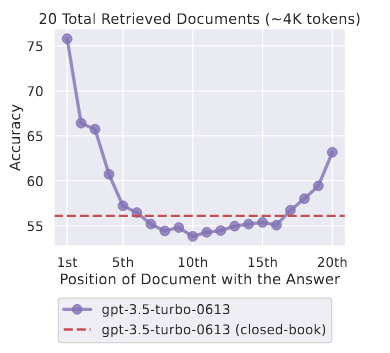
\includegraphics[scale=0.9]{images/Lost_in_the_middle.png}
    \caption{Качество ответа в зависимости от положения релевантной информации в контексте, взято из \cite{lost_in_the_middle}.}
\end{figure}

% Возникновение такой зависимости вполне закономерно вытекает из того, что большинство обучаемых данных, содержат полезную информацию в основном в начале и конце.

На практике в задаче RAG такая проблема чаще всего решается добавлением в pipeline генерации дополнительной reranker-модели, предназначенной для ранжирования документов, извлеченных из базы знаний retrieval-моделью, на основании их релевантности к запросу.

Такой подход эффективен, однако фундаментально никак не решает существующую проблему. Кроме того, из-за эффекта кумулятивной ошибки, потенциально возникающей при использовании слабых retrieval- и reranker-моделей, даже хорошая генеративная модель может показывать низкое качество по причине неуместного контекста.

\hfill

Способ борьбы с этой проблемой предлагают авторы статьи <<From Artificial Needles to Real Haystacks: Improving
Retrieval Capabilities in LLMs by Finetuning on
Synthetic Data>> \cite{synth_needle}. Они генерируют синтетический датасет из набора словарей и обучают модель находить значение по ключу. 

Дообучение модели на такую прокси-задачу закрепляет навык поиска информации в контексте и почти полностью решает описанную в предыдущей статье проблему. Кроме того, это не ухудшает обобщающую способность -- результаты модели на общих бенчмарках если и упали, то незначительно.

\begin{figure}[h!]
    \centering
    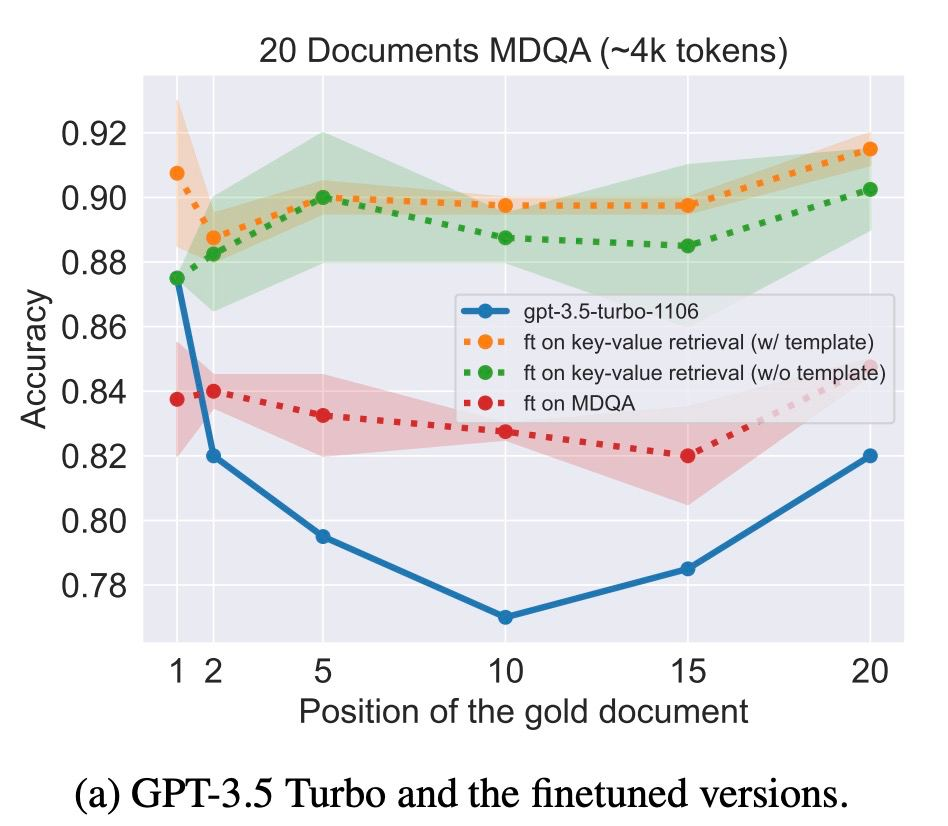
\includegraphics[scale=0.35]{images/artificial_needle_result.jpg}
    \caption{Качество после дообучения, взято из \cite{synth_needle}.}
\end{figure}

\newpage

\subsection{Нерелевантный контекст}
\label{subsec:raft} \index{Chapter4!RAFT}

Как упоминалось ранее, еще одной серьезной проблемой контекстной генерации являются нерелевантные документы. Они могут как просто ухудшать качество ответа, так и приводить к <<галлюцинациям>> модели.

Этот эффект детально описан в статьях <<Large Language Models Can Be Easily Distracted by Irrelevant Context>> \cite{irrelevant_retrieve} и <<Making Retrieval-Augmented Language Models Robust to Irrelevant Context>> \cite{irrelevant_retrieve_ralm}.

\begin{figure}[h!]
    \centering
    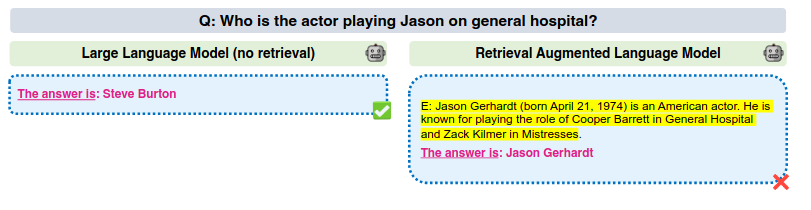
\includegraphics[scale=0.5]{images/hallucinations.png}
    \caption{Неверный ответ из-за нерелеватного контекста, взято из \cite{irrelevant_retrieve_ralm}}
\end{figure}

Кроме изучения негативного влияния, в работе \cite{irrelevant_retrieve_ralm} также приведен способ решения проблемы -- дообучение на датасете со смесью релевантных и нерелевантных документов в контексте. 

\hfill

Духовным наследником этой идеи является исследование <<RAFT: Adapting Language Model to Domain Specific RAG>> \cite{raft}, где описан метод Retrieval Augmented
Fine Tuning (RAFT). Основная идея подхода заключается в дообучении модели на синтетически расширенных датасетах. Авторы предполагают следующую процедуру обработки SFT-датасетов с контекстно-зависимыми запросами:
\begin{enumerate}

  \item \textbf{\textit{Обогащение контекста.}}
  
  К исходному контексту запроса добавляются релевантные фрагменты из других запросов, что позволяет модели научиться работать в условиях, максимально схожих с реальными, и выделять полезные данные в условиях шума.
  
 \item \textit{\textbf{Разметка Chain-of-Thought (CoT).}}
  
  Ответы аннотируются с явным выделением логических цепочек рассуждений. Это позволяет модели учиться обосновывать свой ответ и аргументированно использовать релевантный контекст. Такая разметка делается синтетически при помощи запросов к другой LLM.
  
  \item \textit{\textbf{Добавление негативных примеров.}}
  
  В датасет включаются запросы без релевантных документов, где ожидаемым ответом ставится отказ. Это формирует у модели навык распознавать неподходящий контекст и явно отмечать неспособность предоставить корректный ответ в этой ситуации.
  
\end{enumerate}

Авторы статьи отмечают, что CoT-разметка играет ключевую роль в этом подходе - она не только делает обучение более стабильным, но и существенно увеличивает качество итоговой модели.

\begin{figure}[h!]
    \centering
    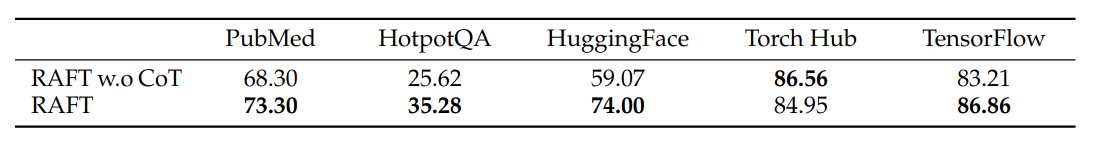
\includegraphics[scale=0.4]{images/raft_cot.png}
    \caption{Влияние CoT, взято из \cite{raft}.}
\end{figure}

Данный подход позволяет адаптировать языковые модели к генерации ответов в условиях шума, а также развивает их способность аргументировать ответы. Глобально этот подход делает этап обучения наиболее близким к реальному сценарию применения модели.

\begin{figure}[h!]
    \centering
    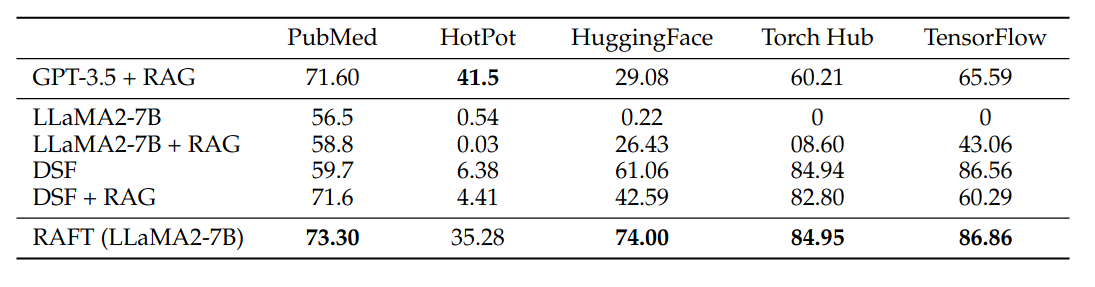
\includegraphics[scale=0.42]{images/raft_result.png}
    \caption{Результаты RAFT, взято из \cite{raft}.}
\end{figure}

\subsection{Построение решения задачи}
\label{sec:Solution} \index{Chapter4!Solution}

Для оптимизации времени разработки эффективного подхода было принято решения разделить процесс обучения на несколько ключевых этапов и в дальнейшем оценить влияние каждого из них.

\begin{enumerate}

  \item \textbf{\textit{Адаптация к русскому языку.}}

    Современные языковые модели обучаются на обширных мультиязычных текстовых корпусах, что обеспечивает их базовую функциональность во многих сценариях применения. Однако доминирование англоязычных данных в обучающих выборках приводит в выраженному ухудшению качество генерации и понимания для языков с меньшей репрезентацией, включая русский.
  
 \item \textit{\textbf{Улучшение качества контекстно-зависимой генерации.}}
  
    Следующим этапом стал сравнительный анализ различных подходов адаптации языковой модели к задаче контекстной генерации. Главной целью было сравнение классического подхода и RAFT. 
  
  \item \textit{\textbf{Адаптация к большому контексту.}}
  
    Для решения проблемы <<lost in the middle>> \cite{lost_in_the_middle}, а также увеличения размера эффективного контекста модели, было проведено сравнительное дообучение на синтетических данных с размером контекста порядка 7-8 тысяч токенов.
  
\end{enumerate}

\newpage
